\begin{frame} \frametitle{\vspace*{0.5cm}Interface response to a 10 MPa US pulse}
  \begin{figure}
    \centering
    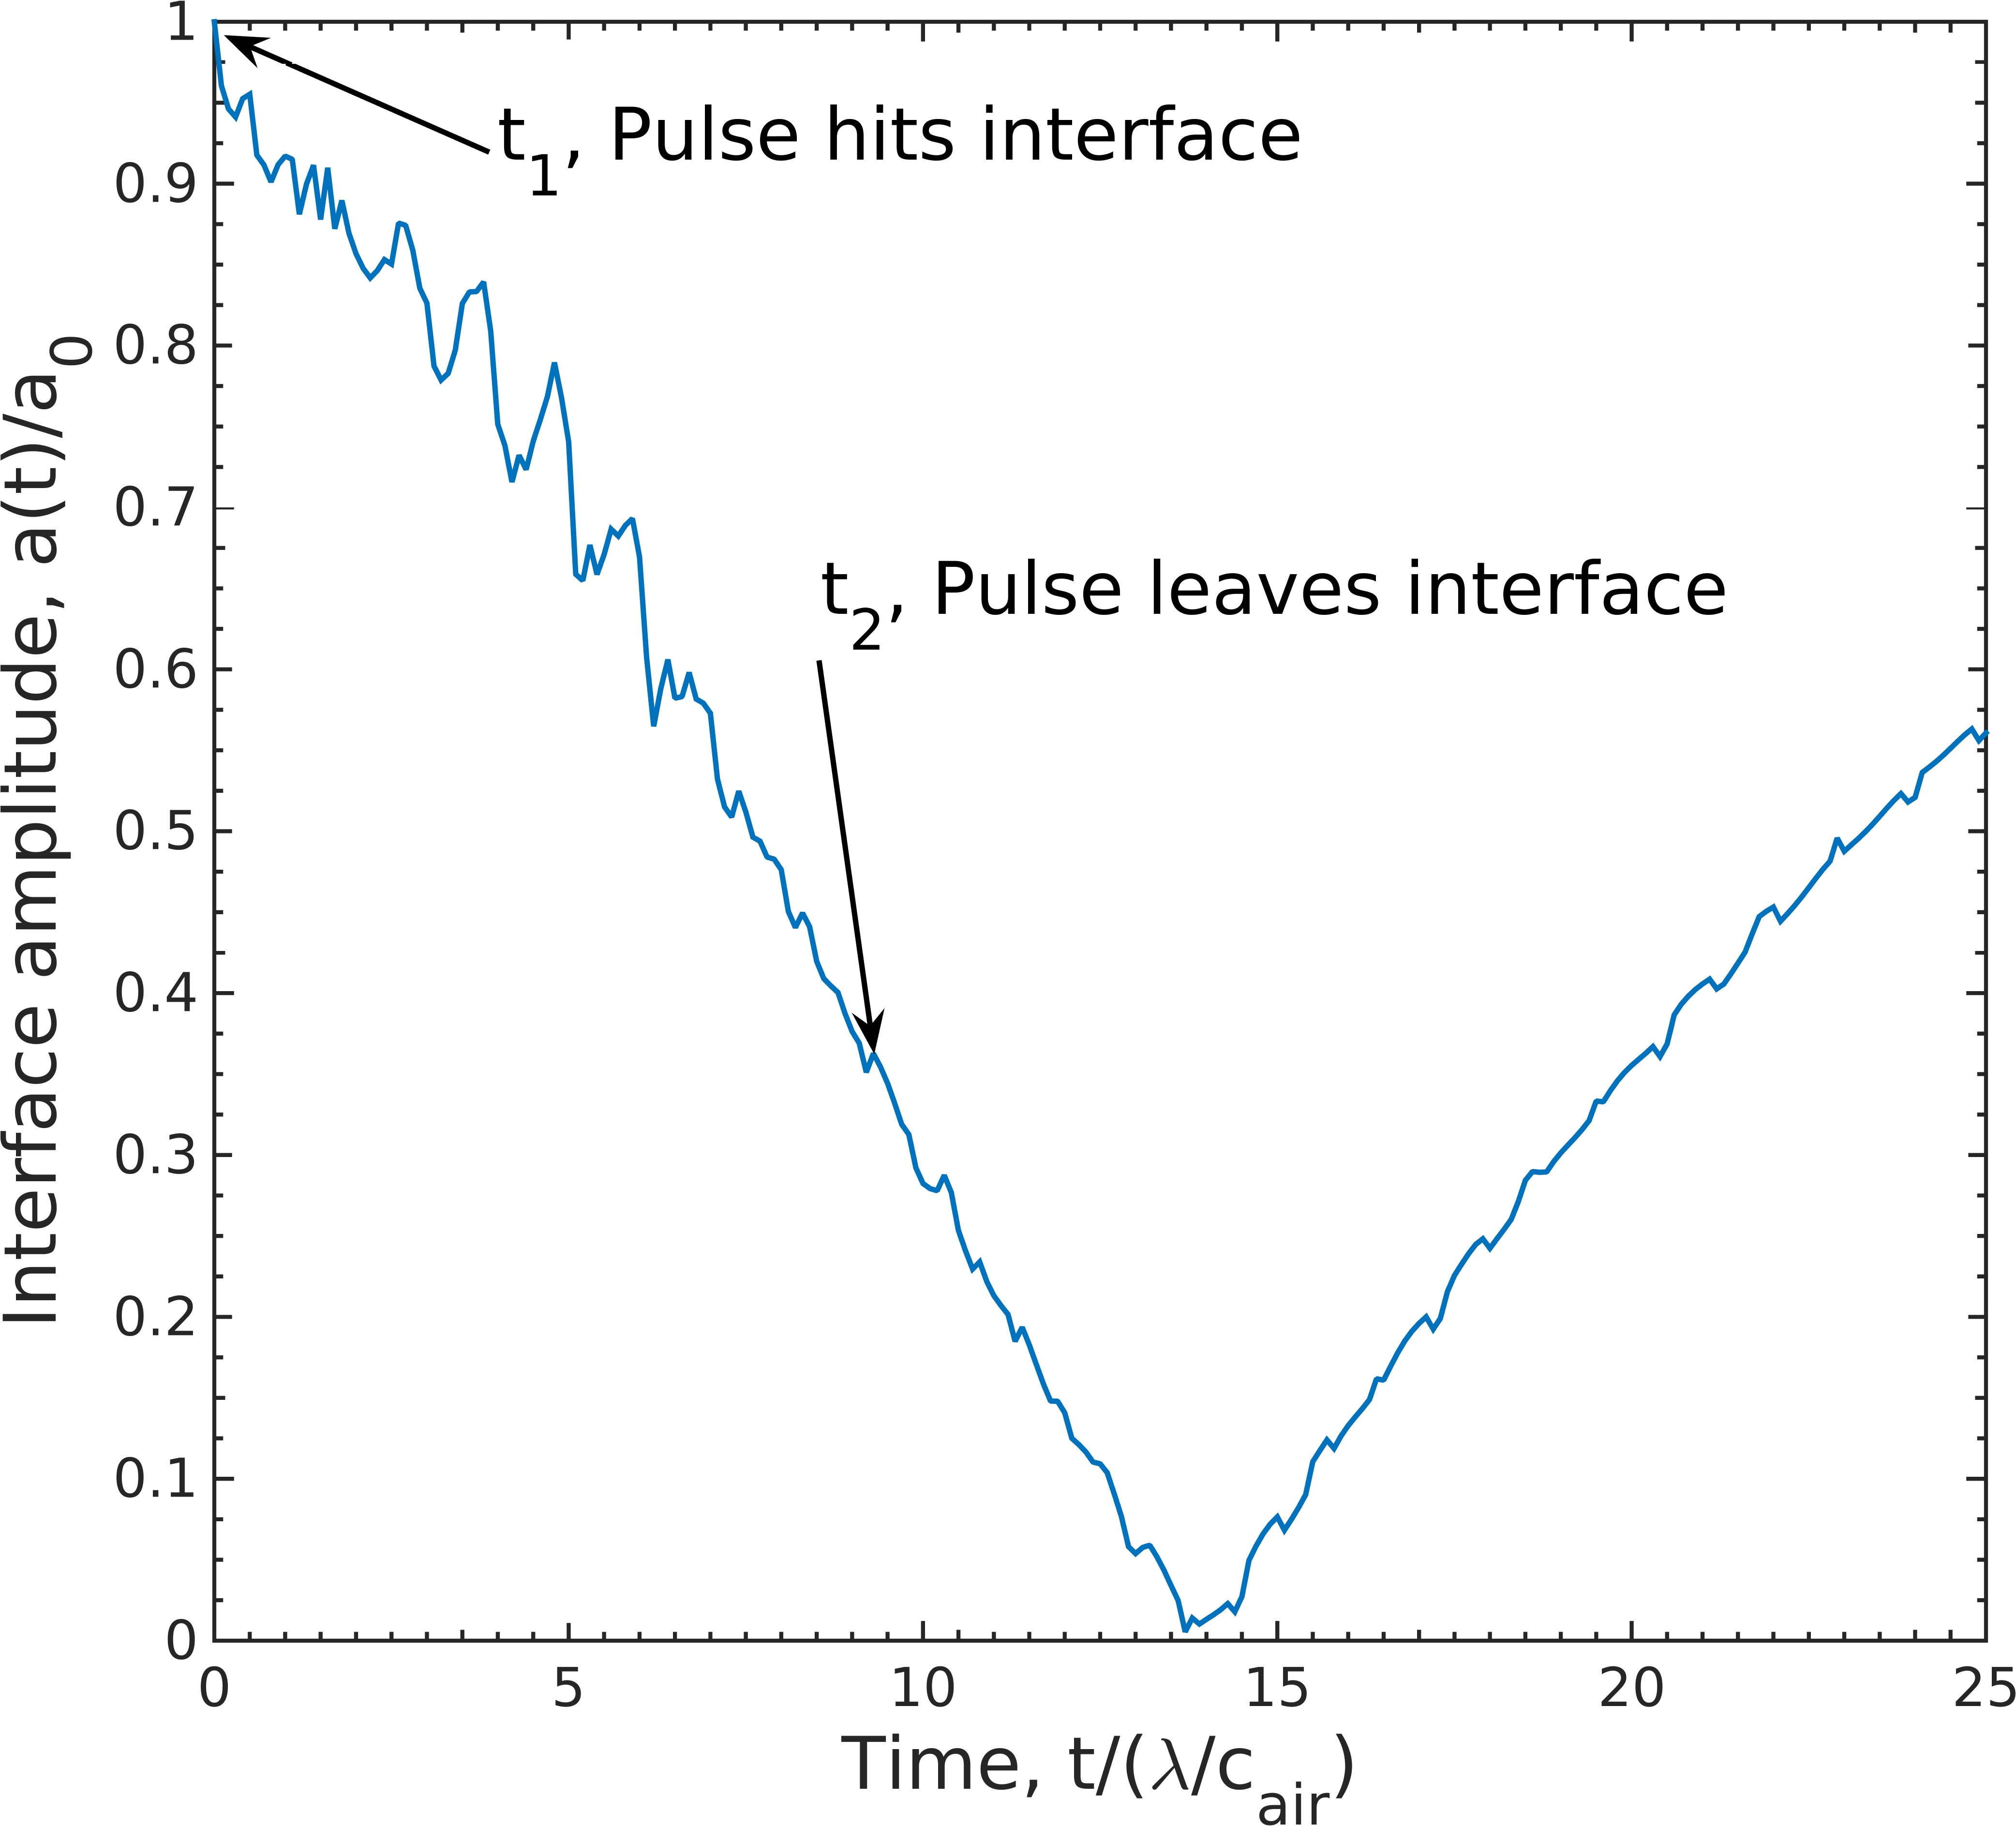
\includegraphics[width=0.48\textwidth]{../figs/lung_figs/us_intf_schematic}\hfill
    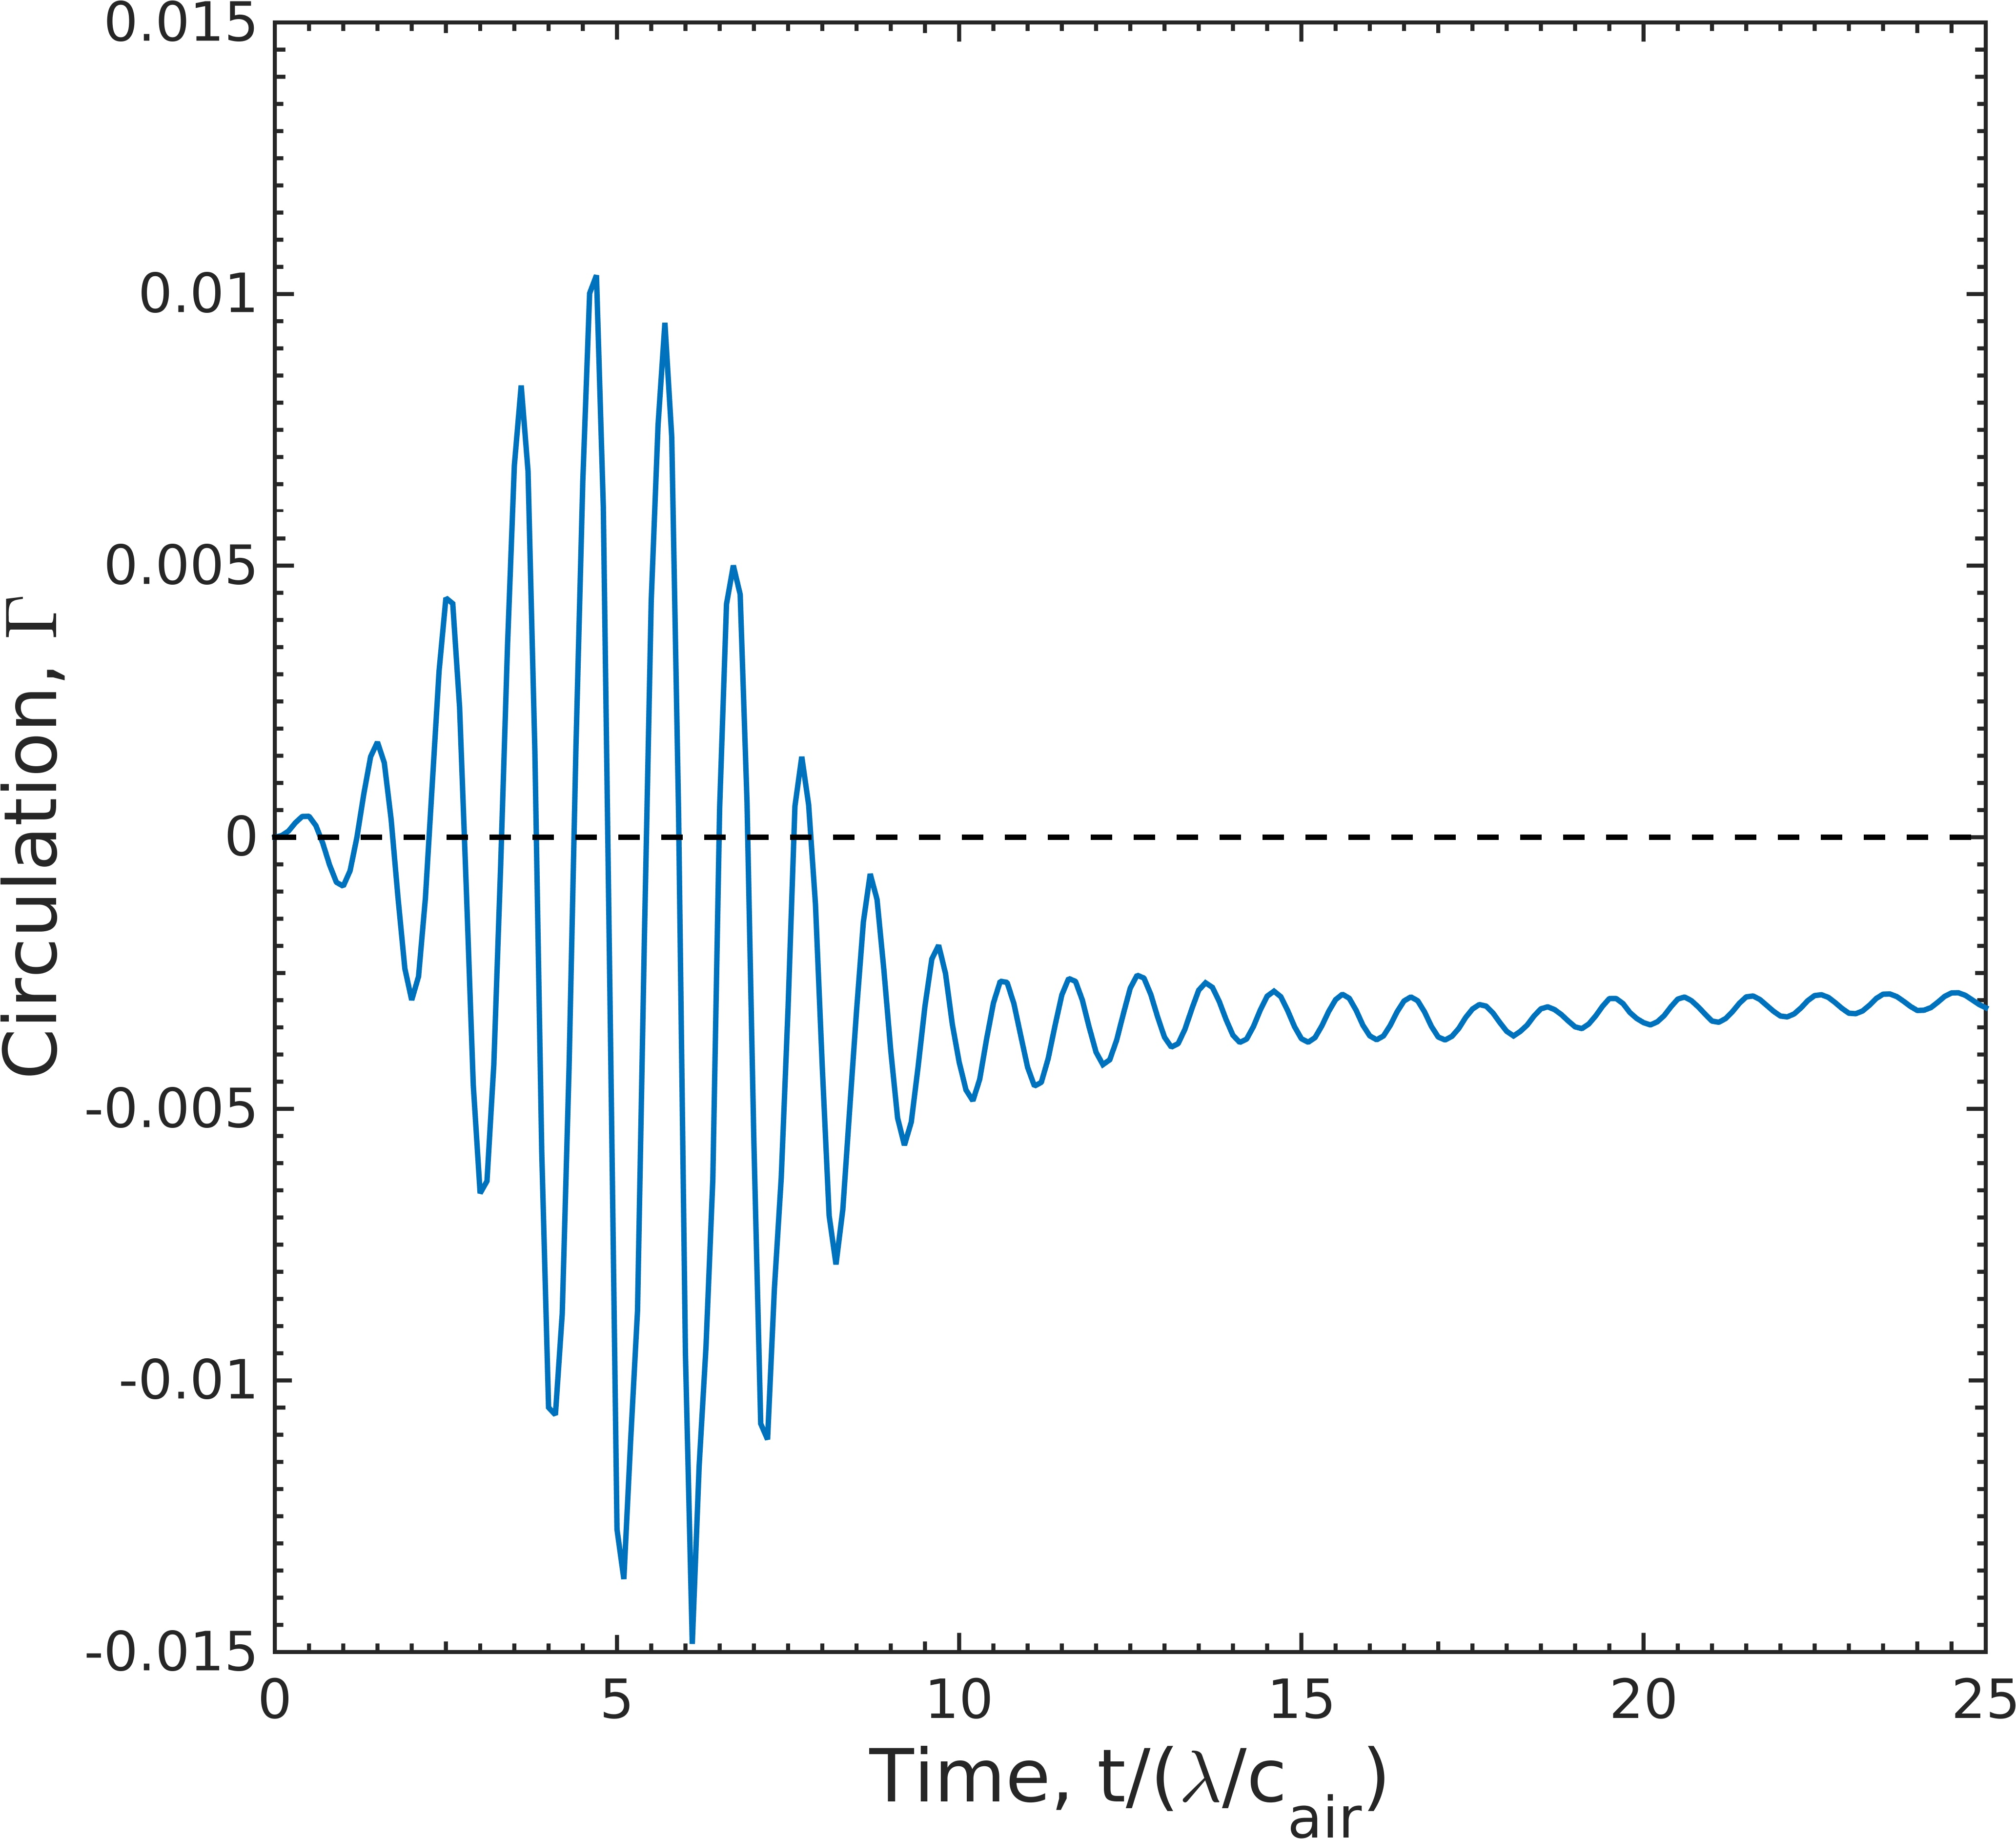
\includegraphics[width=0.48\textwidth]{../figs/lung_figs/us_circ_schematic}
  \end{figure}
  \begin{itemize}
  \item Qualitatively, the interface response for the 10 MPa US pulse looks very similar to the 10 MPa trapezoidal wave. 
  \item The circulation deposited is of the same order as the equivalent amplitude trapezoidal wave.
  \end{itemize}
\end{frame}
%%% Local Variables:
%%% mode: latex
%%% TeX-master: "../main"
%%% End:
